\section{Additional Simulation Results}
\label{appendix-simulation-figures}
Table~\ref{tab:pmm-k-sensitivity-supp} summarizes the reported
\(n=2000\) PMM donor-width sensitivity cells.  Coverage of \(\beta^\ast\)
remains close to nominal across the reported donor-width
scales, whereas coverage of the data-generating coefficient decreases
as the smooth donor law spreads probability over more distant donors.
This pattern is consistent with a change in the PMM point-estimator
target as the donor-width scale increases.
\begin{table}[ht]
\centering
\scriptsize
\setlength{\tabcolsep}{4pt}
\begin{tabular}{rllrrrr}
\toprule
\(k\) &
\makecell{Imputation\\counts \(m\)} &
\makecell{Mean effective\\donor count} &
\makecell{Mean donor-pool\\probability mass} &
\makecell{Mean SE /\\empirical SD} &
\makecell{Coverage\\\(\beta^\ast\)} &
\makecell{Coverage\\\(\beta_0\)}\\
\midrule
5  & 5, 25, 50, 100 & 11.2 & 0.59 & 1.03--1.31 & 0.954--0.979 & 0.934--0.968\\
10 & 5, 25, 50, 100 & 19.0 & 0.66 & 1.00--1.10 & 0.946--0.956 & 0.923--0.944\\
20 & 5, 25, 50      & 32.5 & 0.73 & 0.97--1.02 & 0.943--0.953 & 0.888--0.913\\
30 & 5, 25, 50      & 44.6 & 0.77 & 1.00--1.01 & 0.946--0.952 & 0.862--0.886\\
\bottomrule
\end{tabular}
\caption{Reported \(n=2000\) RW-PMM donor-width sensitivity
summary.  Entries are ranges across the imputation counts shown in the
second column.  Donor-pool probability mass is the probability the
smooth law assigns to the \(k\) donors in the hard rule's donor pool.}
\label{tab:pmm-k-sensitivity-supp}
\end{table}
Figure~\ref{fig:gs-pmm-current-n2000-supp} shows the same \(n=2000\)
RW-PMM validation cells graphically across donor-width scales.
Only cells with complete 2500-replicate results are plotted; \textcolor{blue}{empty cells still running}.
\begin{figure}[ht]
\centering
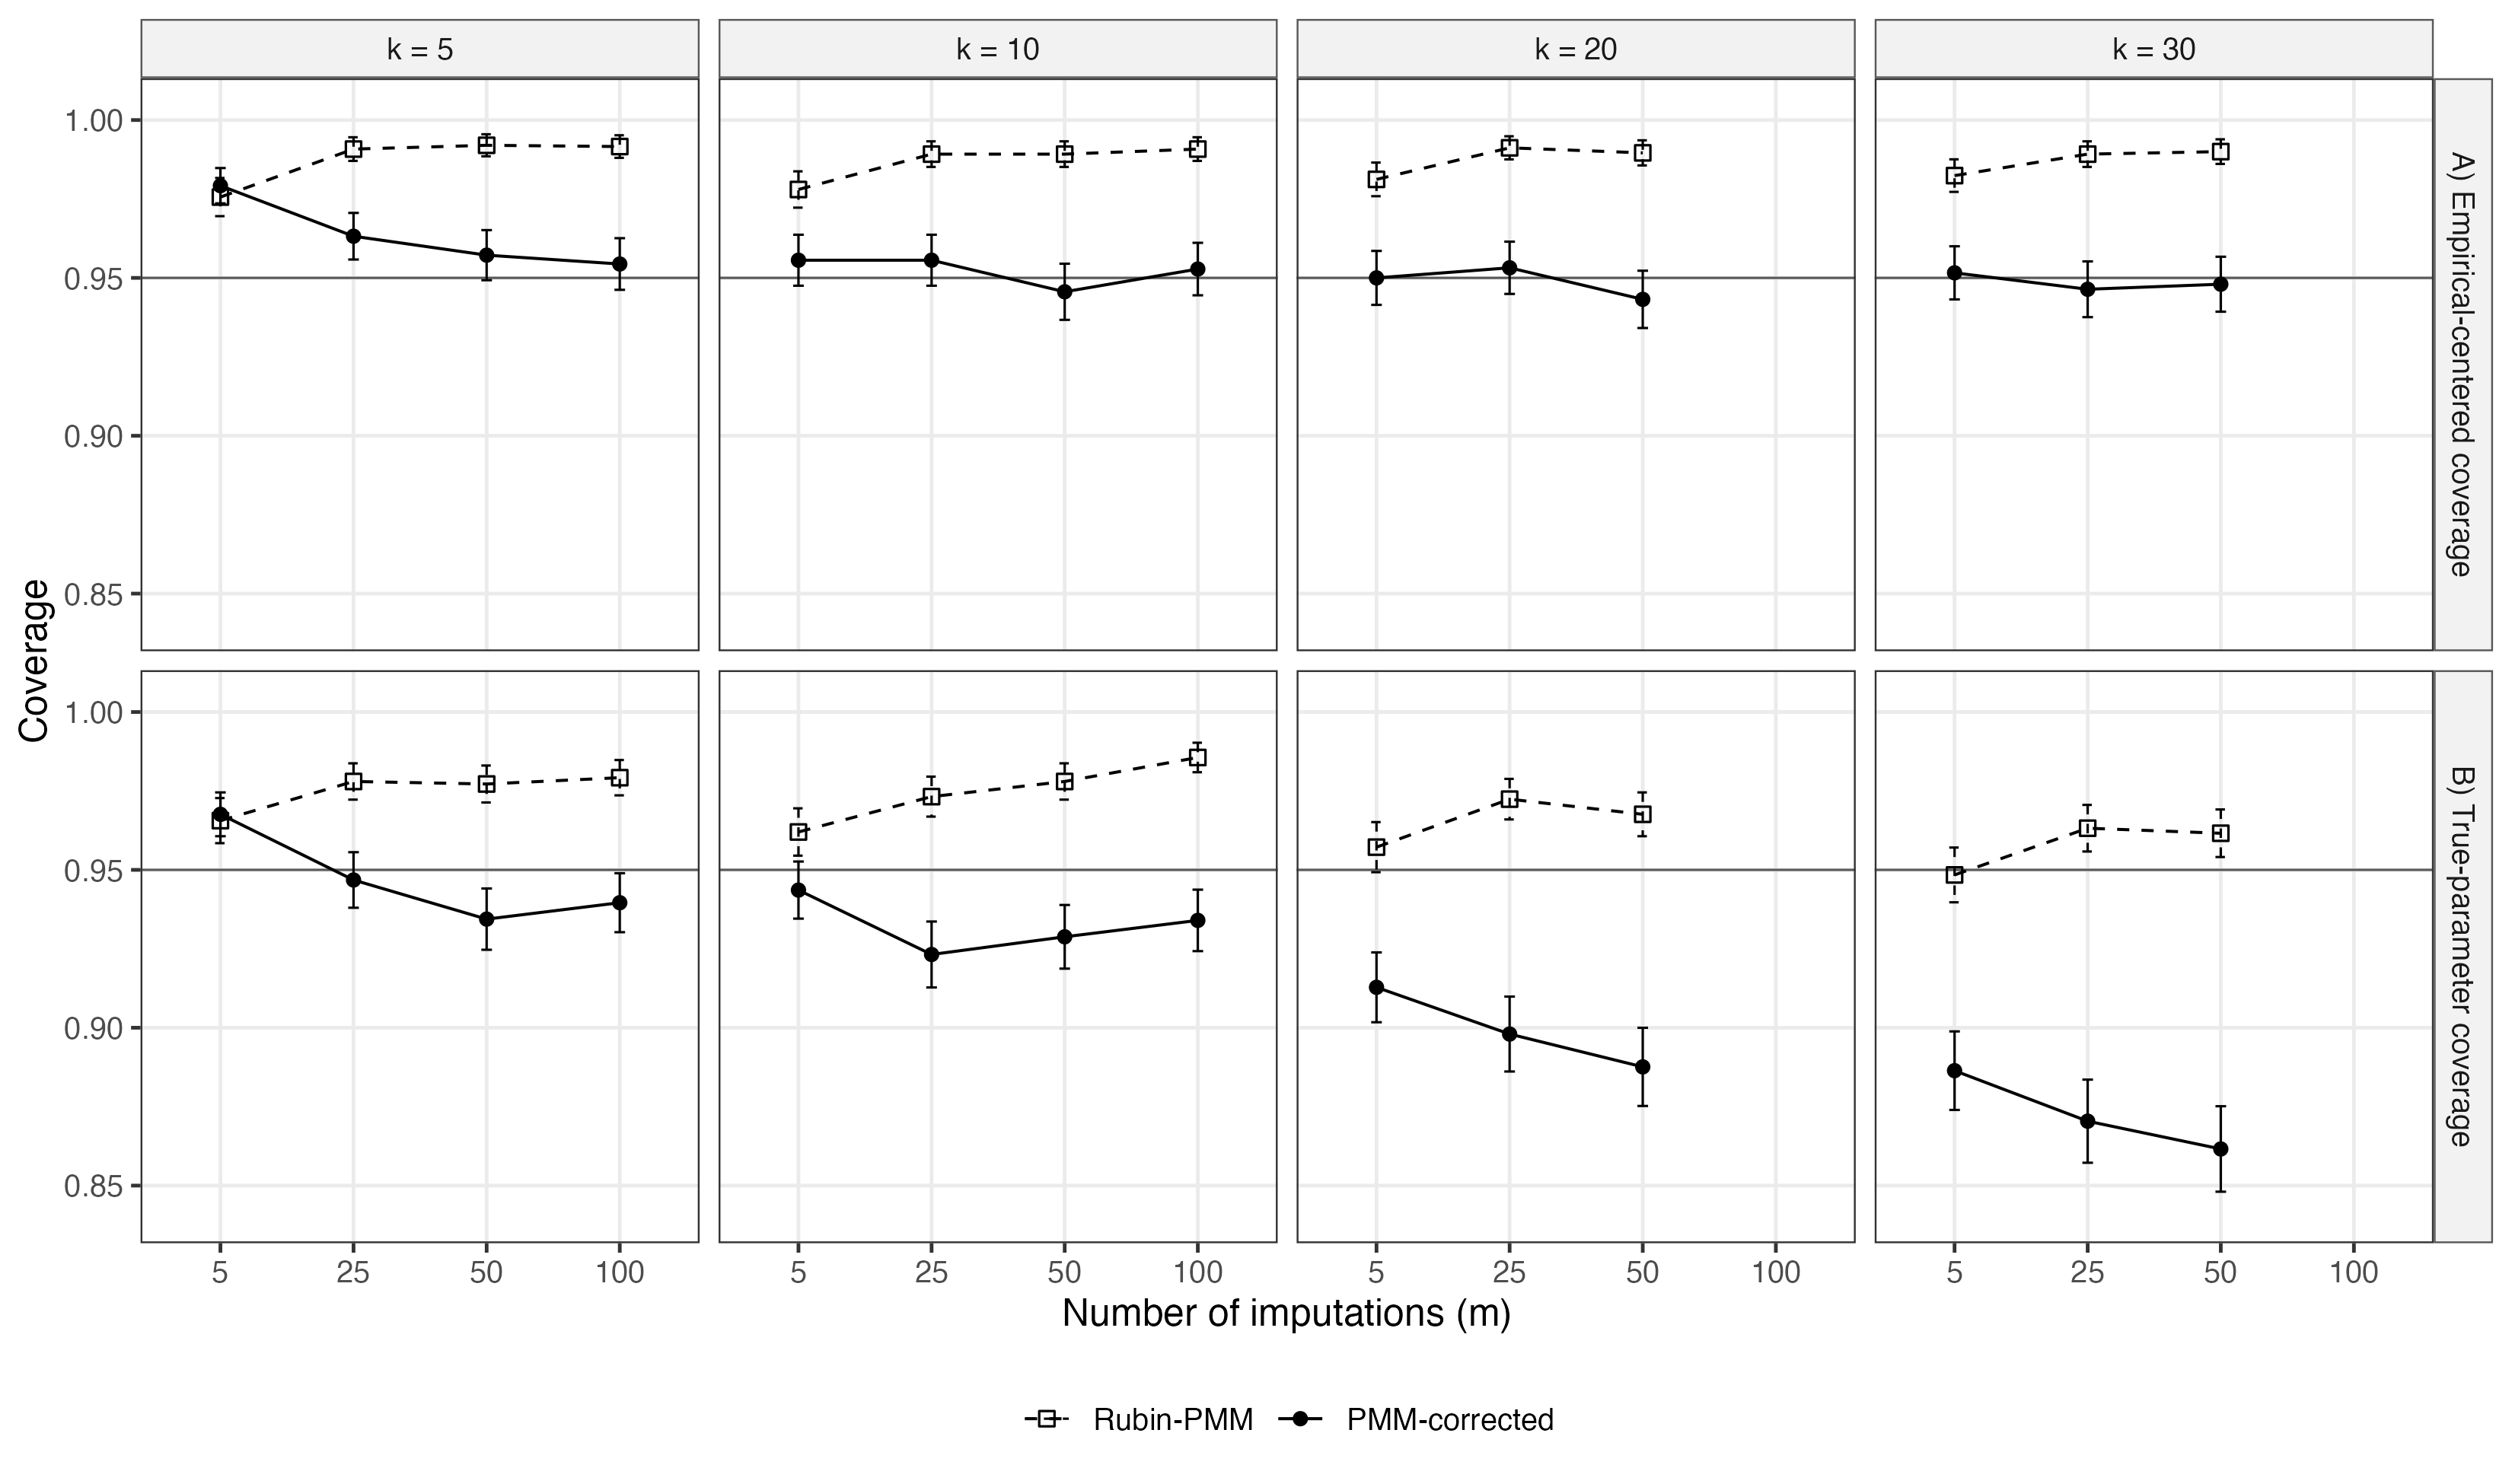
\includegraphics[width=\textwidth]{figures/gs_pmm_current_coverage_n2000.png}
\caption{RW-PMM measurement-error validation results at
\(n=2000\), shown across donor-width scales \(k\).  Rows distinguish
coverage of \(\beta^\ast\) from coverage of \(\beta_0\).  Empty points
mark simulation cells not included in the present result set.}
\label{fig:gs-pmm-current-n2000-supp}
\end{figure}
Figure~\ref{fig:gs-pmm-current-k5-supp} shows the available
RW-PMM validation cells graphically for donor-width scale
\(k=5\) across sample sizes.  Only cells with complete 2500-replicate
results are plotted.
\begin{figure}[ht]
\centering
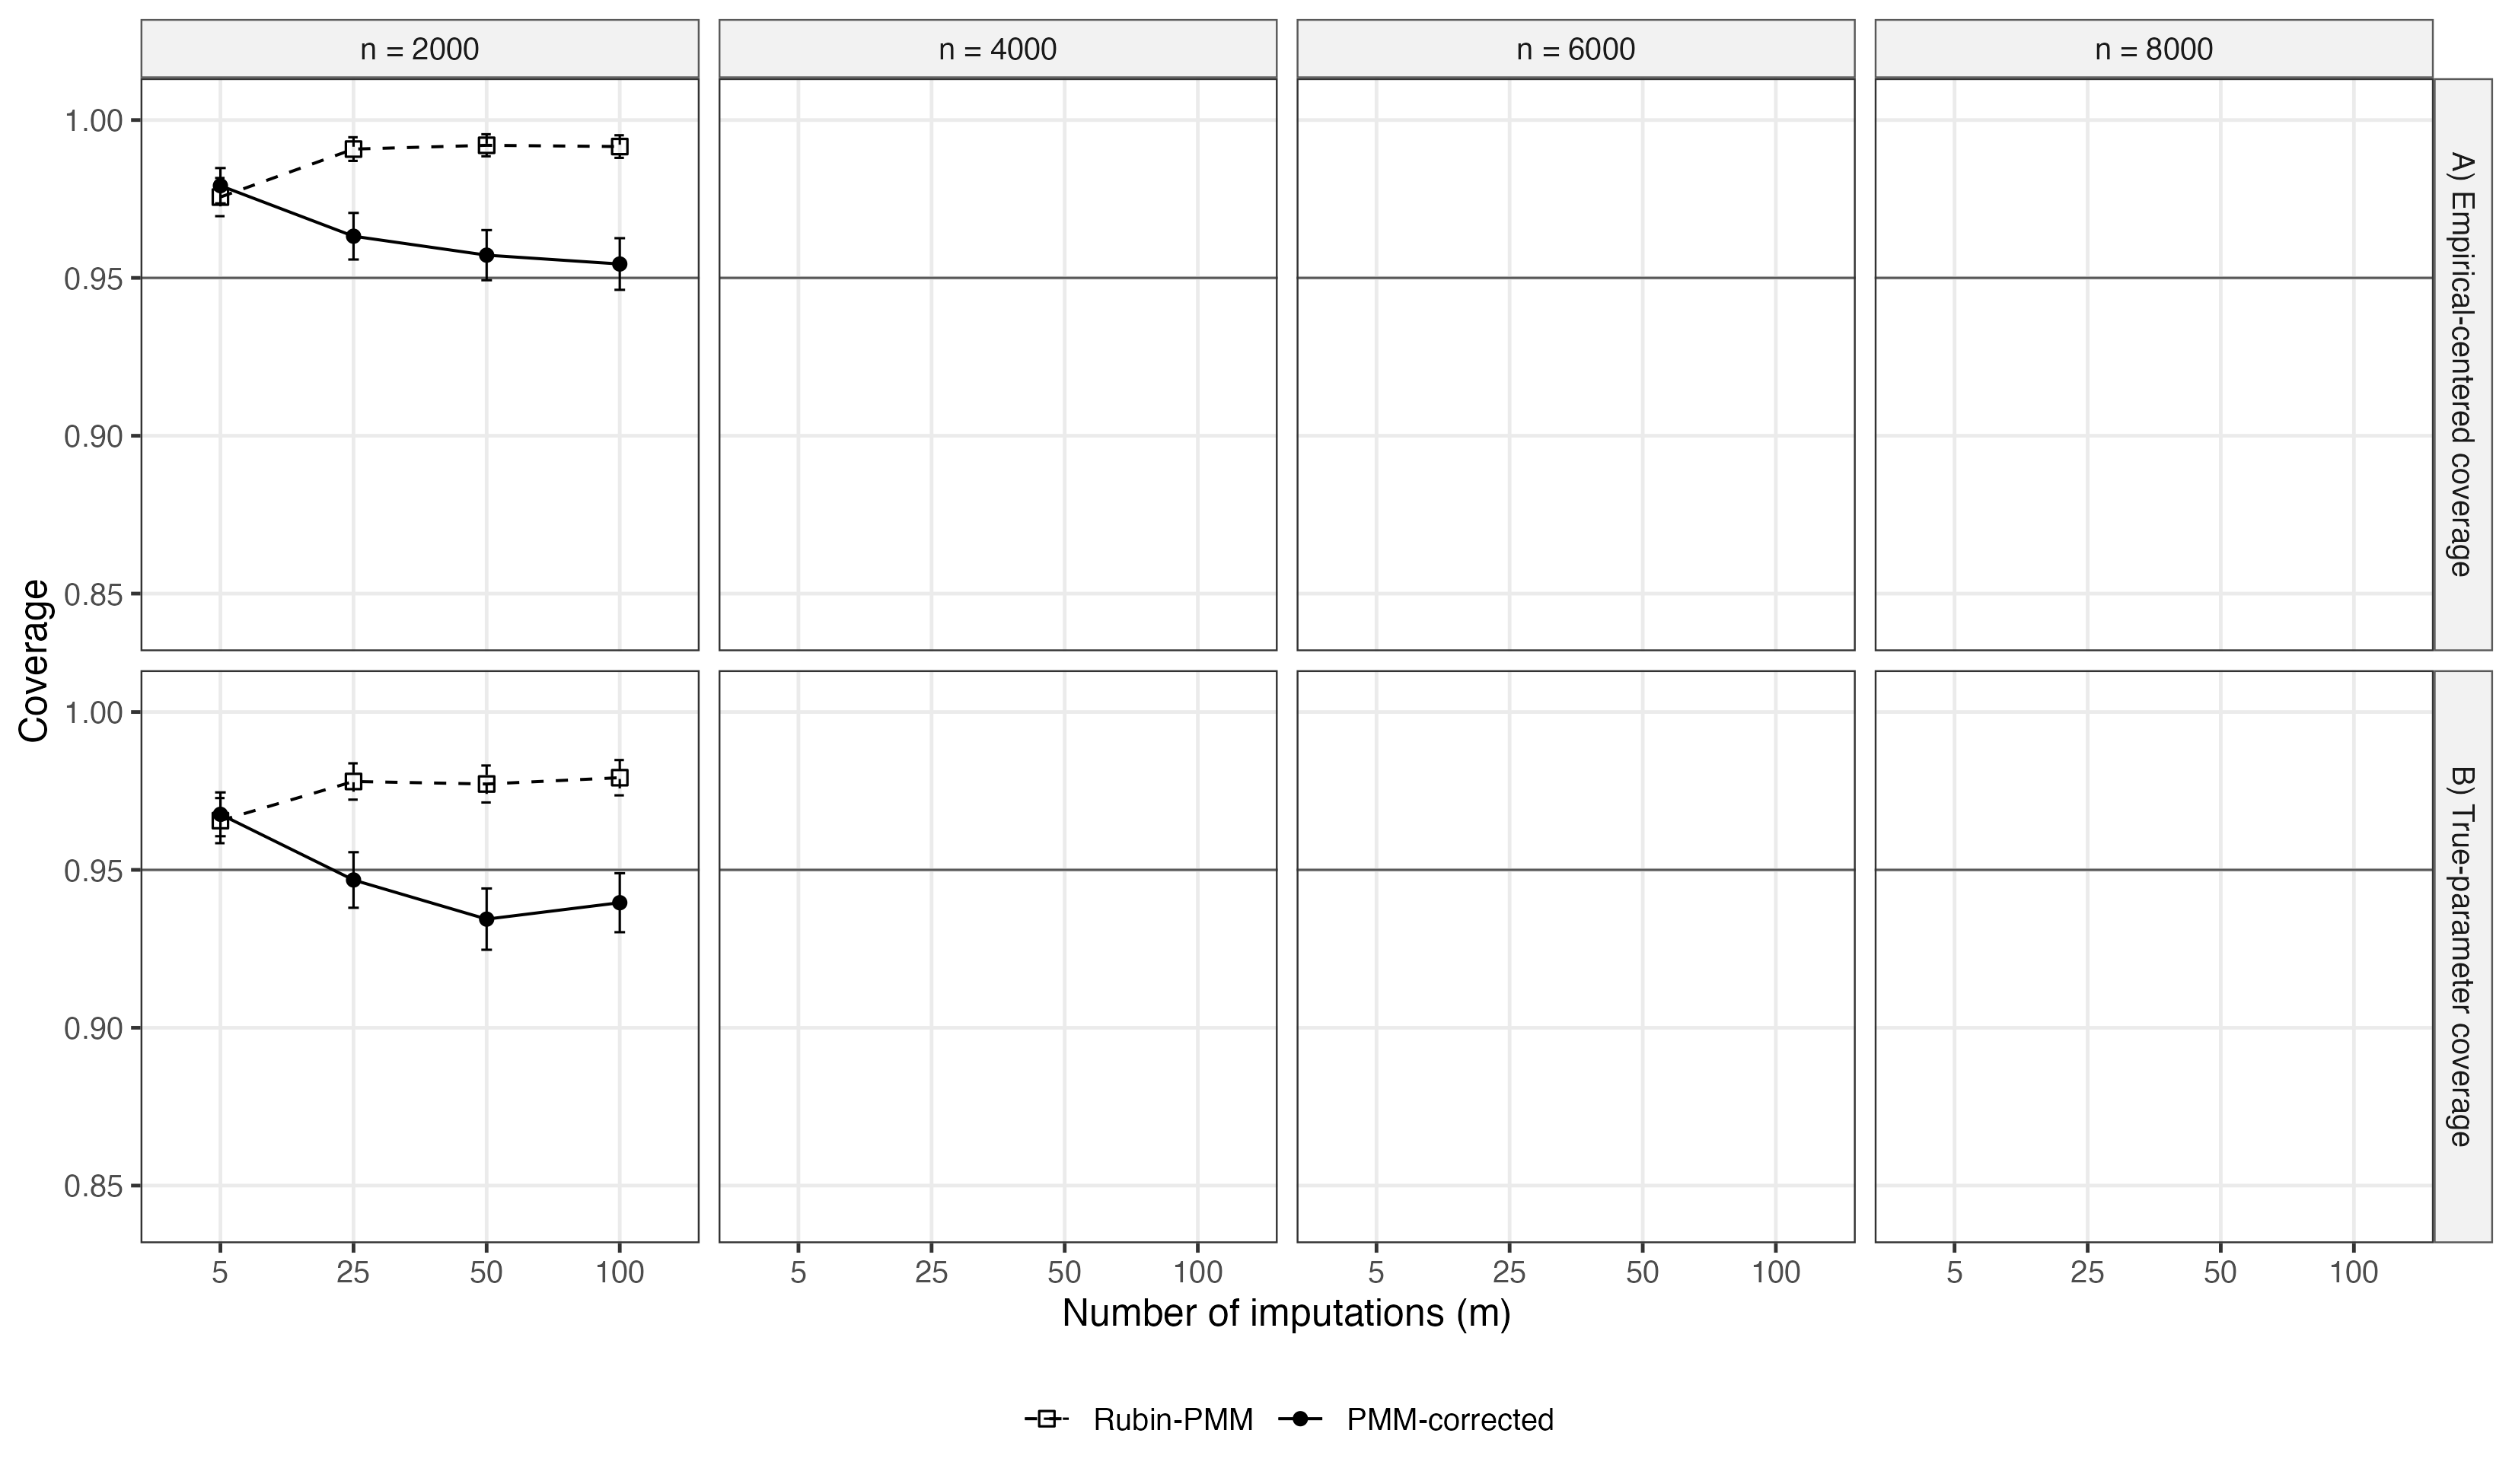
\includegraphics[width=\textwidth]{figures/gs_pmm_current_coverage_k5_by_n.png}
\caption{RW-PMM measurement-error validation results
for donor-width scale \(k=5\).  Columns show sample size \(n\), and
rows distinguish coverage of \(\beta^\ast\) from coverage of
\(\beta_0\).  Empty panels mark simulation cells not included in the
present result set.}
\label{fig:gs-pmm-current-k5-supp}
\end{figure}
For the parametric validation analysis, the main text focuses on the
original Giganti--Shepherd sample size \(n=4000\).
Figure~\ref{fig:gs-parametric-full-supp} shows the full parametric
measurement-error grid for \(n\in\{2000,4000,6000,8000\}\), which is
summarized in the main text only at \(n=4000\).
\begin{figure}[ht]
\centering
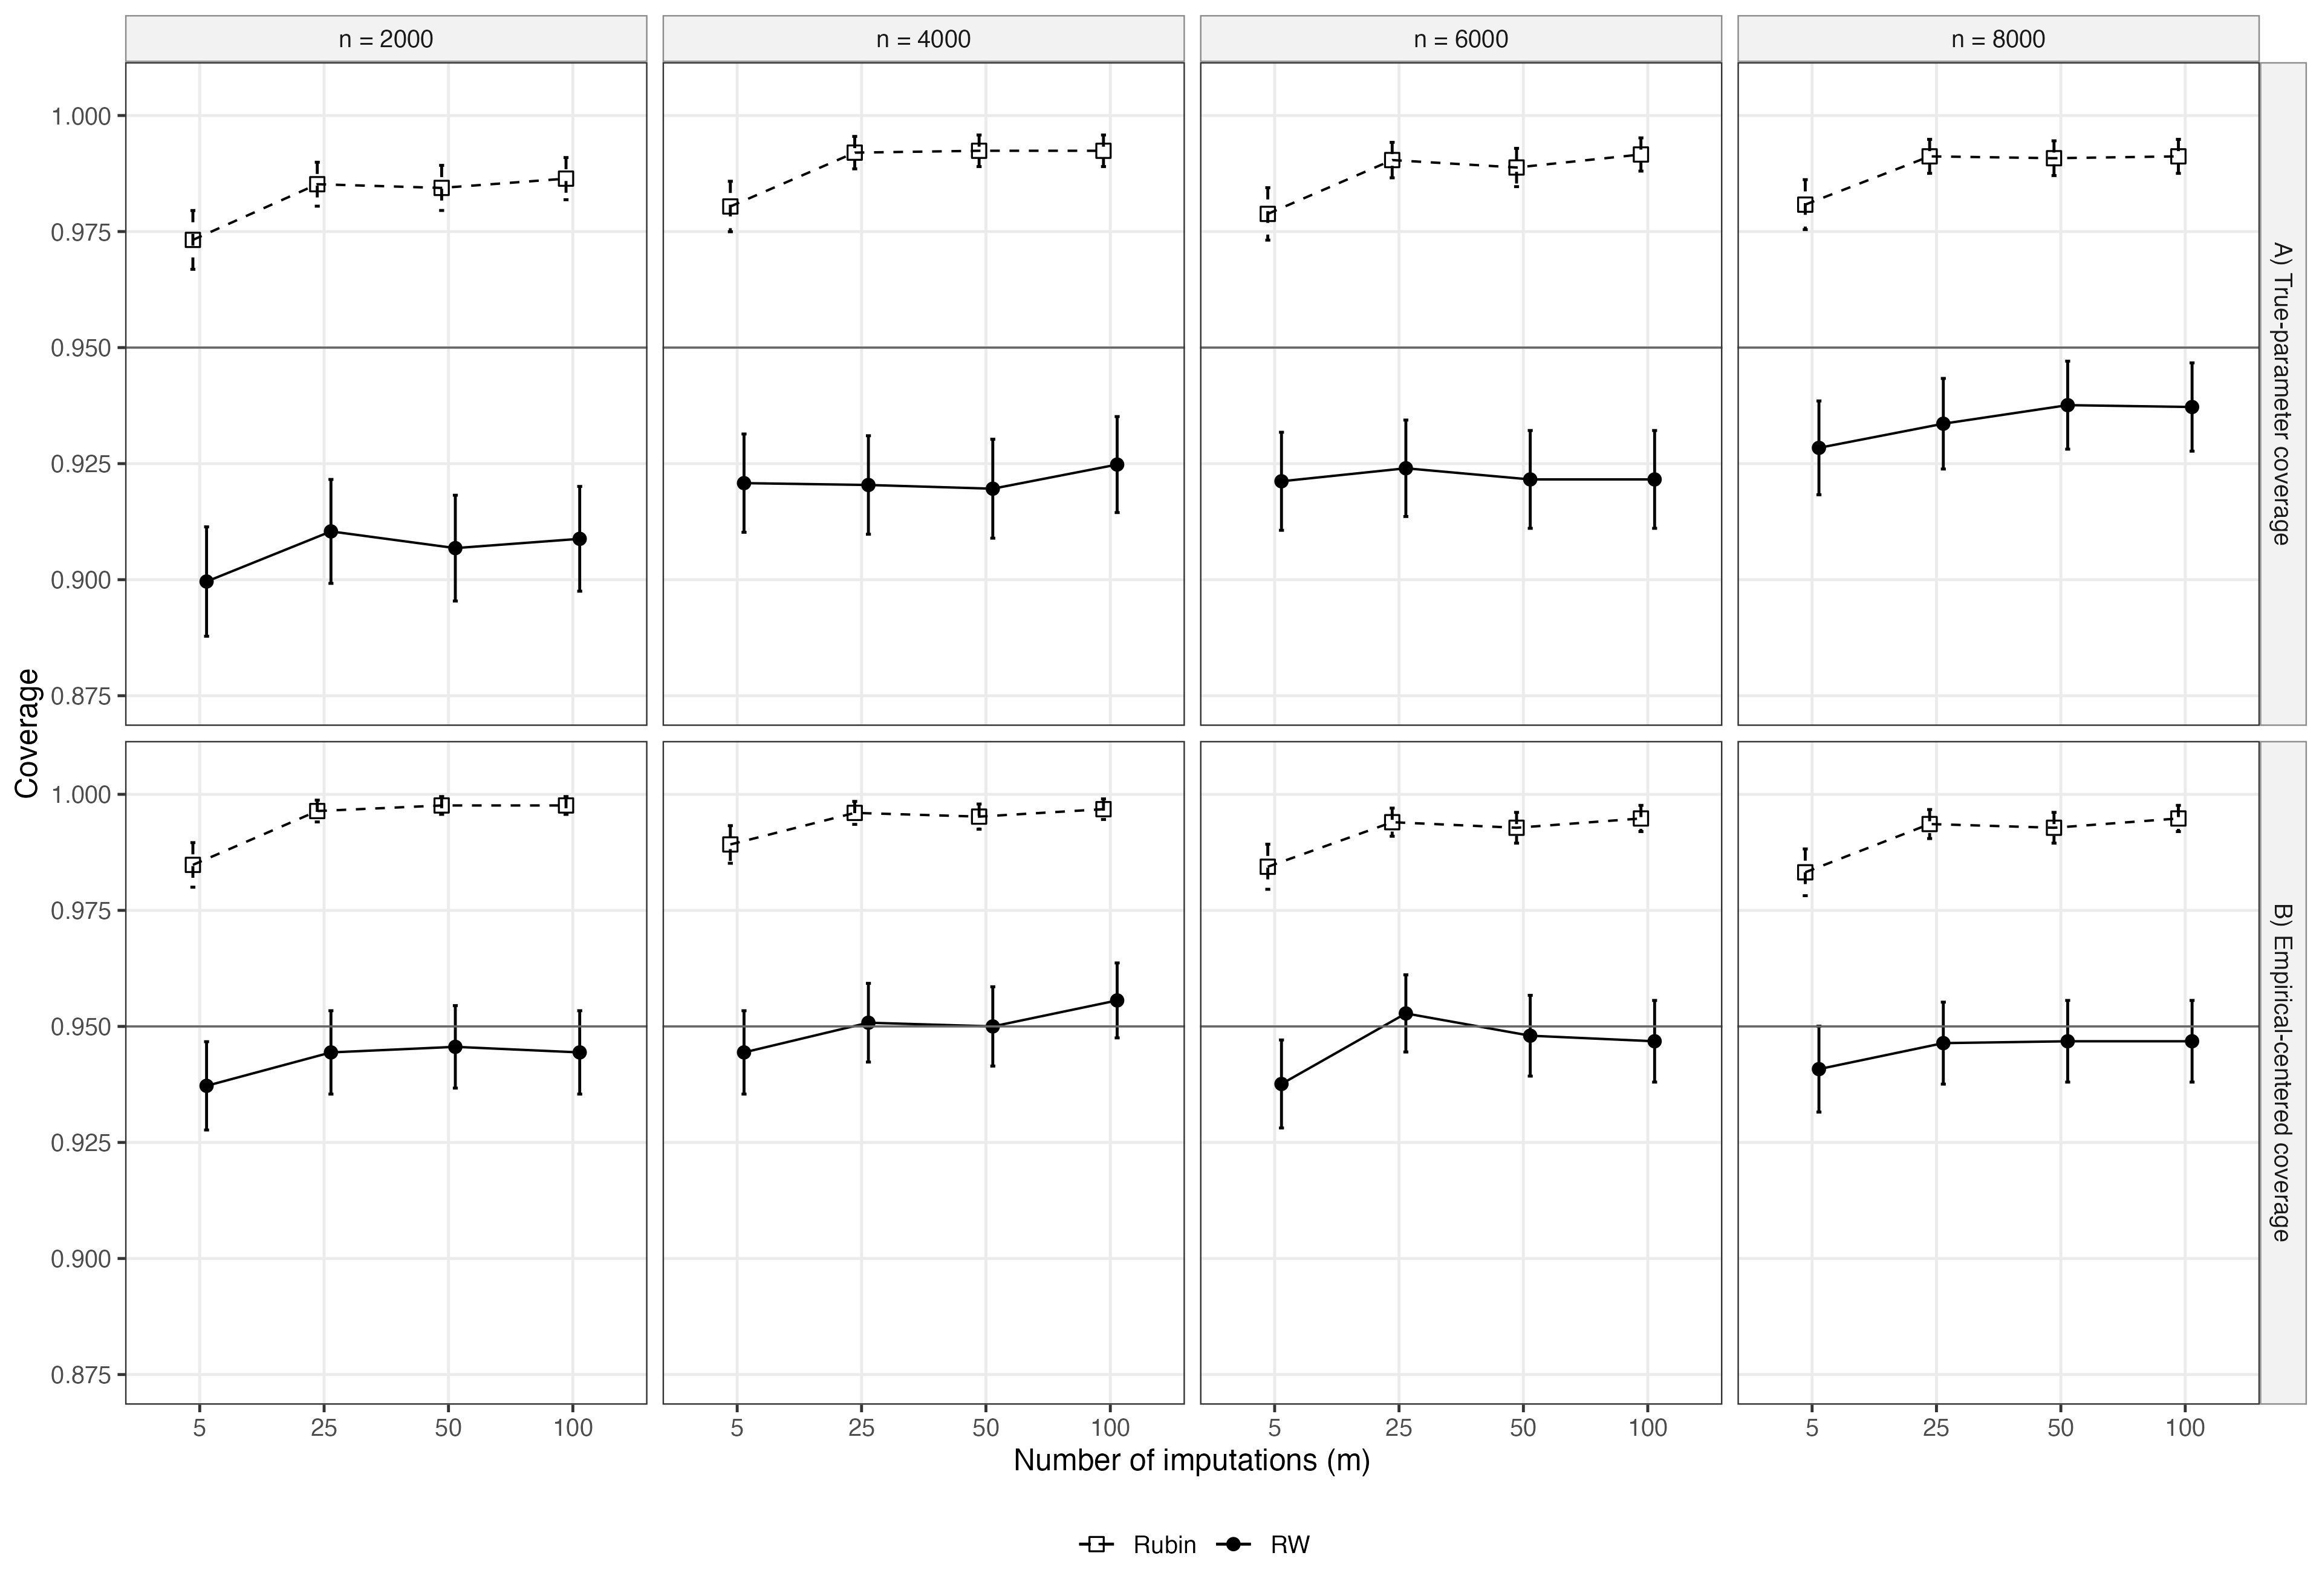
\includegraphics[width=\textwidth]{figures/gs_parametric_coverage.png}
\caption{Full parametric MICE measurement-error simulation grid. Rows
show coverage of \(\beta_0\) and coverage of \(\beta^\ast\) for the
chained conditional MICE implementation. The main text focuses on
\(n=4000\), matching the original Giganti--Shepherd sample size.}
\label{fig:gs-parametric-full-supp}
\end{figure}
\clearpage